\newpage
\section{Sidebands}
\label{sec:sidebands}

\todo[inline]{Update these plots with detector uncertainties and run 4a+5 when available.}

To validate the modelling of neutrino interactions in MicroBooNE and predicted sources of background, several sidebands are employed. These consist of the events selected by the muon neutrino constraint selection, events containing two or more reconstructed showers to study the $\pi^0$ induced backgrounds and shower energy estimation, and near/far sidebands created with combinations of higher energy/lower BDT scoring events. The selection used to obtain the near/far sidebands will be detailed in Sections~\ref{sec:FarSideband} and~\ref{sec:NearSideband}. The following sections only contain a sampling of the distributions inspected during these checks, a more complete set may be found in Appendix~\ref{appendix:SidebandValidations}.

\subsection{$\nu_{\mu}$ Events}
\label{sec:NuMuSideband}

This sideband is obtained by applying the full muon neutrino event selection described in Section~\ref{sec:EventSelections}.

\begin{figure}[H]
    \centering
    \begin{subfigure}{0.33\linewidth}
        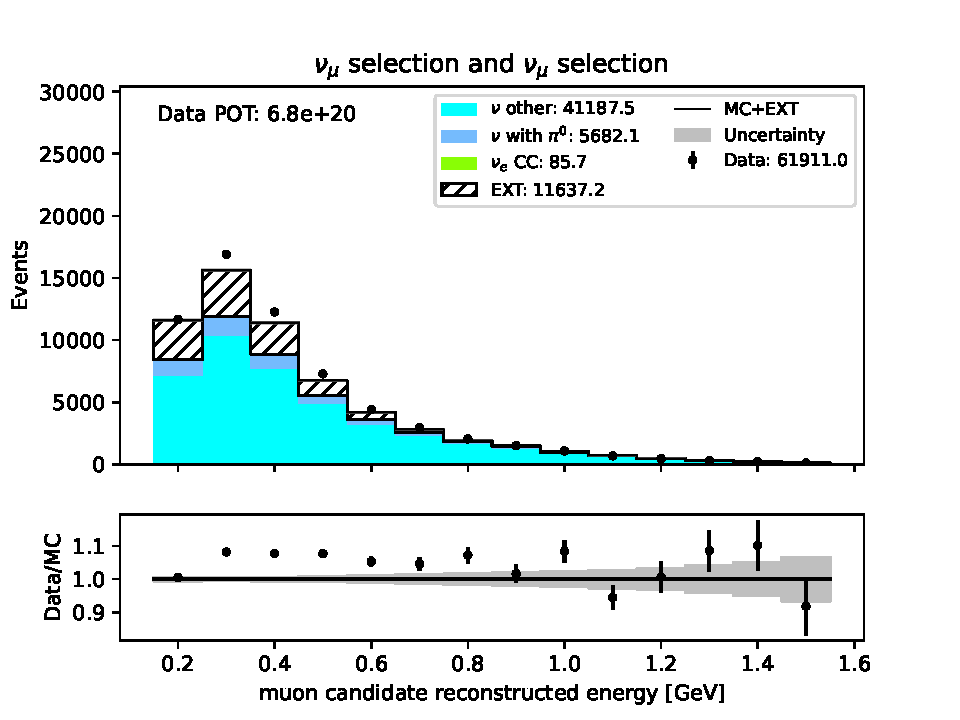
\includegraphics[width=\linewidth]{technote/Sidebands/Figures/NuMuSideband/muon_sideband_muon_energy_run123_NUMU_NUMU.pdf}
        \caption{Muon reconstructed energy.}
    \end{subfigure}%
    \begin{subfigure}{0.33\linewidth}
        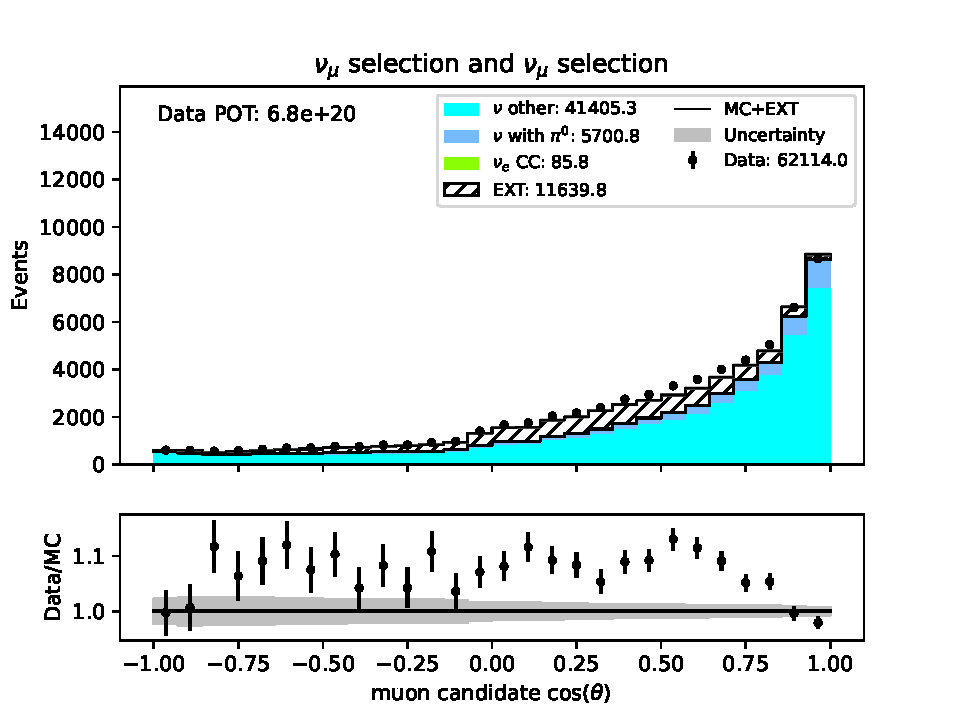
\includegraphics[width=\linewidth]{technote/Sidebands/Figures/NuMuSideband/muon_sideband_muon_theta_run123_NUMU_NUMU.pdf}
        \caption{Muon candidate direction.}
    \end{subfigure}%
    \begin{subfigure}{0.33\linewidth}
        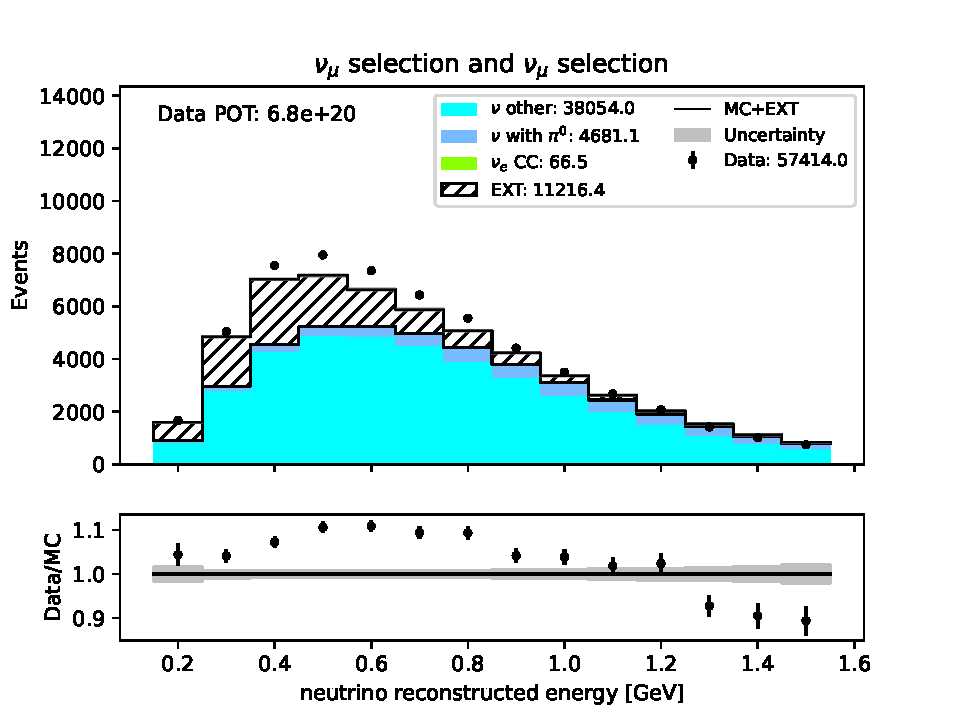
\includegraphics[width=\linewidth]{technote/Sidebands/Figures/NuMuSideband/muon_sideband_neutrino_energy_run123_NUMU_NUMU.pdf}
        \caption{Reconstructed neutrino energy.}
    \end{subfigure}
    \caption{Data and MC simulation comparisons after applying the muon sideband selection from Appendix~\ref{appendix:NuMuSelection}. Data from runs 1, 2, and 3 are shown.}
\end{figure}

\begin{figure}[H]
    \centering
    \begin{subfigure}{0.33\linewidth}
        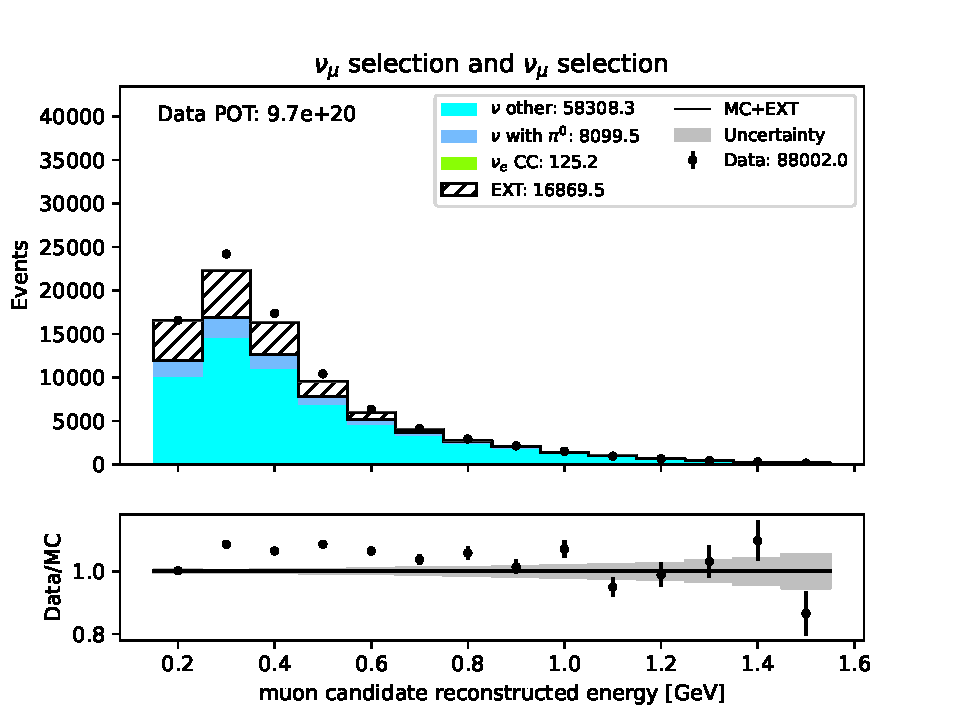
\includegraphics[width=\linewidth]{technote/Sidebands/Figures/NuMuSideband/muon_sideband_muon_energy_run1234b4c4d_NUMU_NUMU.pdf}
        \caption{Muon reconstructed energy.}
    \end{subfigure}%
    \begin{subfigure}{0.33\linewidth}
        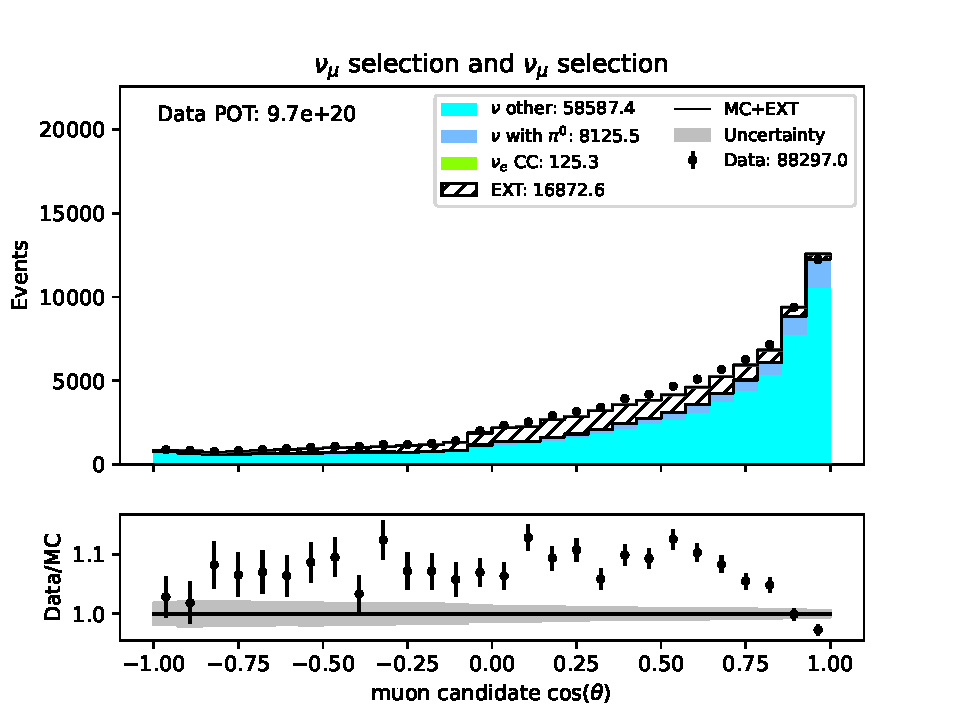
\includegraphics[width=\linewidth]{technote/Sidebands/Figures/NuMuSideband/muon_sideband_muon_theta_run1234b4c4d_NUMU_NUMU.pdf}
        \caption{Muon candidate direction.}
    \end{subfigure}%
    \begin{subfigure}{0.33\linewidth}
        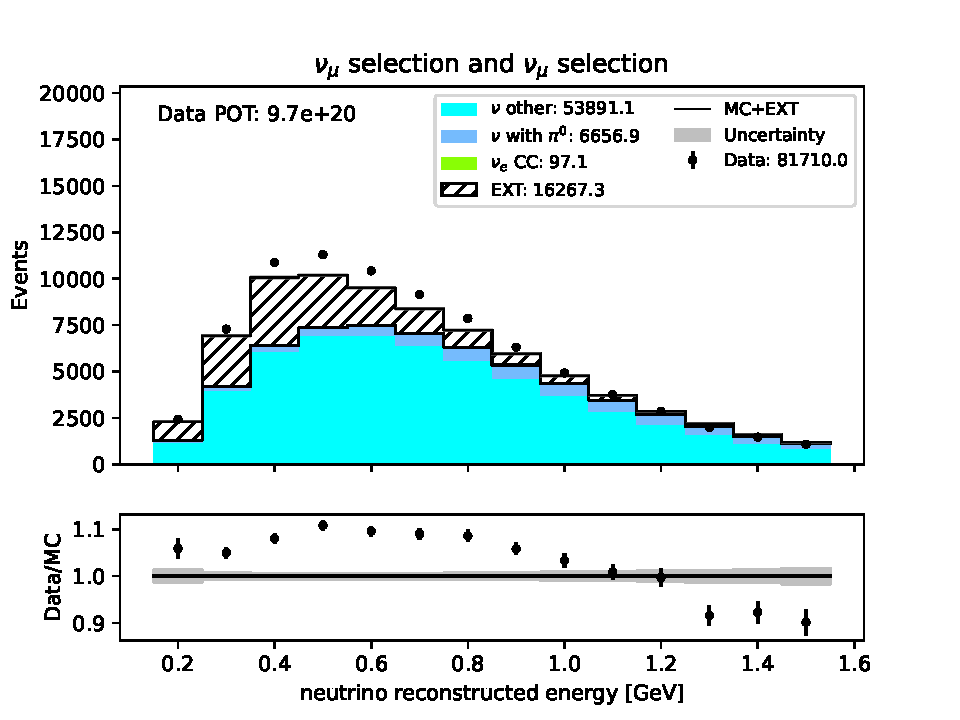
\includegraphics[width=\linewidth]{technote/Sidebands/Figures/NuMuSideband/muon_sideband_neutrino_energy_run1234b4c4d_NUMU_NUMU.pdf}
        \caption{Reconstructed neutrino energy.}
    \end{subfigure}
    \caption{Data and MC simulation comparisons after applying the muon sideband selection from Table~\ref{appendix:NuMuSelection}. Data from runs 1-5 are shown.}
\end{figure}

\subsection{Two Shower Sideband}
\label{sec:TwoShowerSideband}

This sideband is chosen to better understand the detector response to electromagnetic showers and the background induced by neutral pion production.

\todo[inline]{Find out why the "no uncontained showers" cut isn't used any more, and what the pi0 gammadot variable is.}

No pion background scaling is applied to the following plots.

\begin{figure}[H]
    \centering
    \begin{subfigure}{0.33\linewidth}
        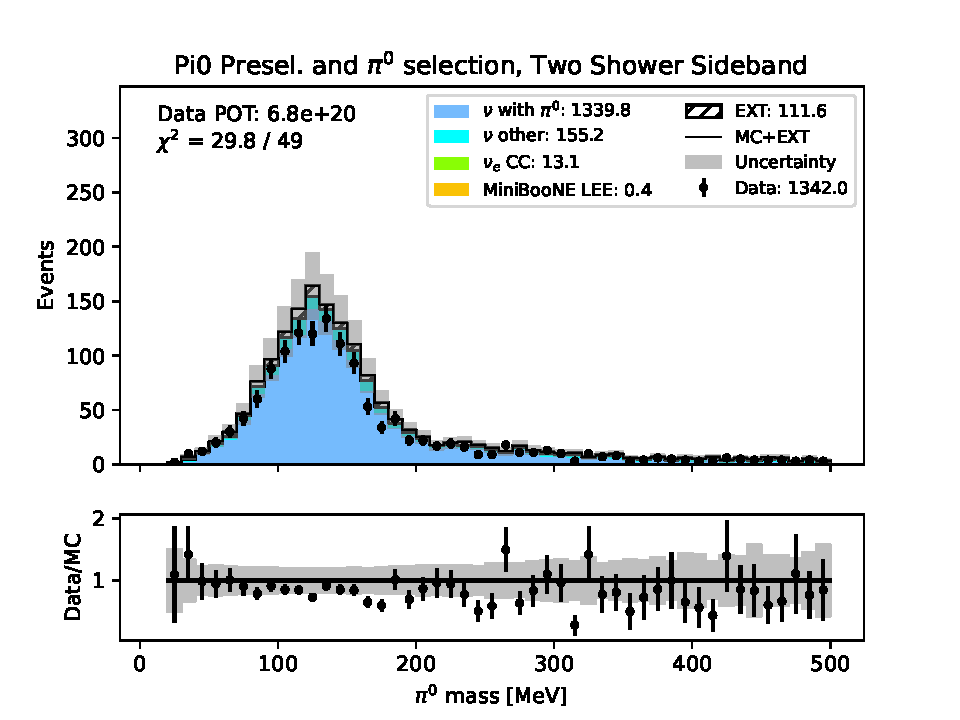
\includegraphics[width=\linewidth]{technote/Sidebands/Figures/TwoShowerSideband/two_shr_sideband_pi0_mass_Y_corr_run123_PI0_PI0.pdf}
        \caption{Reconstructed $\pi^0$ mass.}
    \end{subfigure}%
    \begin{subfigure}{0.33\linewidth}
        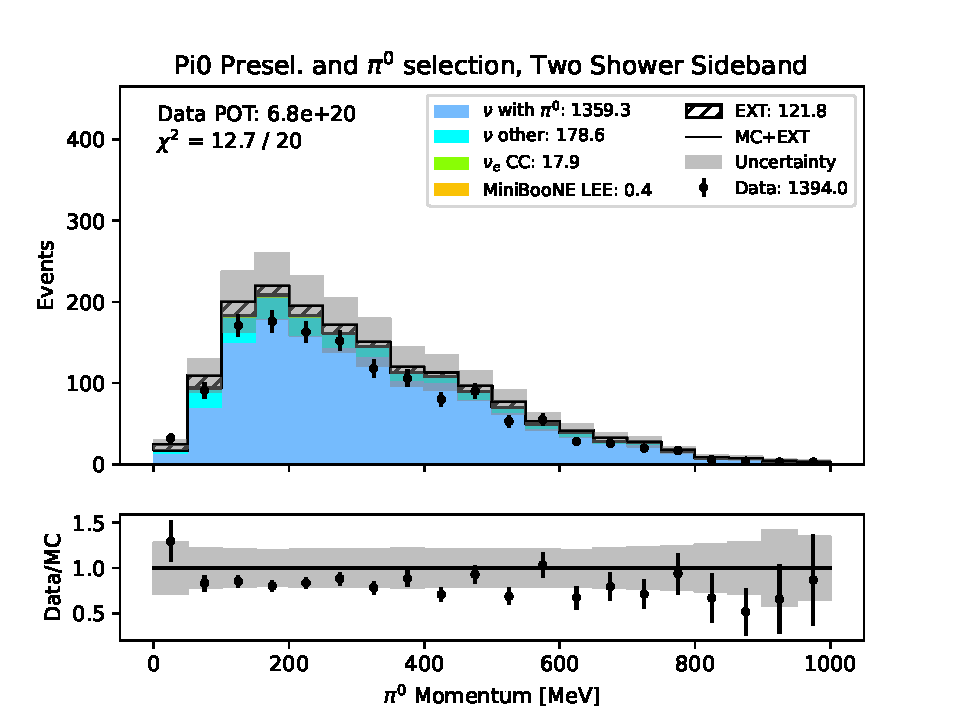
\includegraphics[width=\linewidth]{technote/Sidebands/Figures/TwoShowerSideband/two_shr_sideband_pi0momentum_run123_PI0_PI0.pdf}
        \caption{Reconstructed $\pi^0$ momentum.}
    \end{subfigure}%
    \begin{subfigure}{0.33\linewidth}
        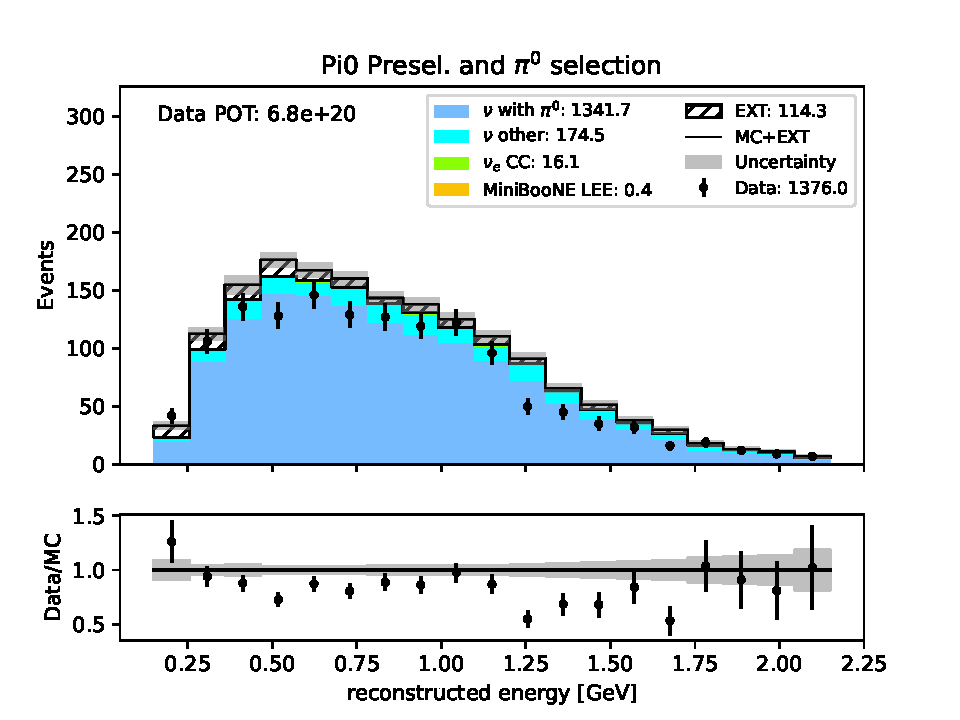
\includegraphics[width=\linewidth]{technote/Sidebands/Figures/TwoShowerSideband/two_shr_sideband_reco_e_run123_PI0_PI0.pdf}
        \caption{Reconstructed neutrino energy.}
    \end{subfigure}
    \caption{Data and MC simulation comparisons after applying the full $\pi^0$ selection from Appendix~\ref{appendix:Pi0Selection} to data from the two shower sideband. Data from runs 1, 2, and 3 are shown.}
    \label{fig:Pi0SidebandRuns123}
\end{figure}

\begin{figure}[H]
    \centering
    \begin{subfigure}{0.33\linewidth}
        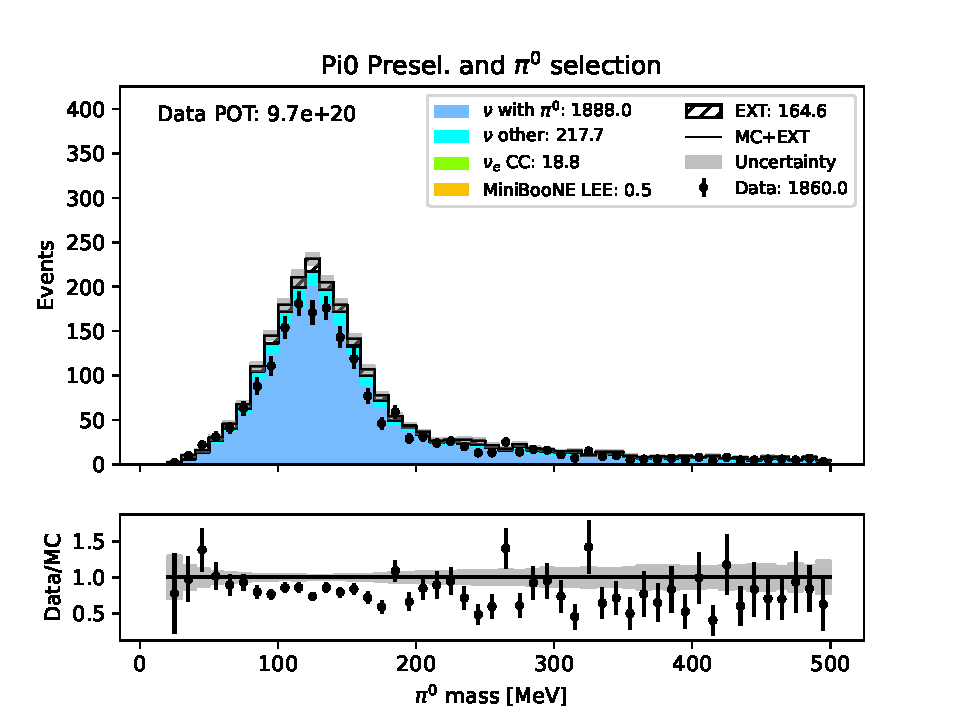
\includegraphics[width=\linewidth]{technote/Sidebands/Figures/TwoShowerSideband/two_shr_sideband_pi0_mass_Y_corr_run1234b4c4d_PI0_PI0.pdf}
        \caption{Reconstructed $\pi^0$ mass.}
    \end{subfigure}%
    \begin{subfigure}{0.33\linewidth}
        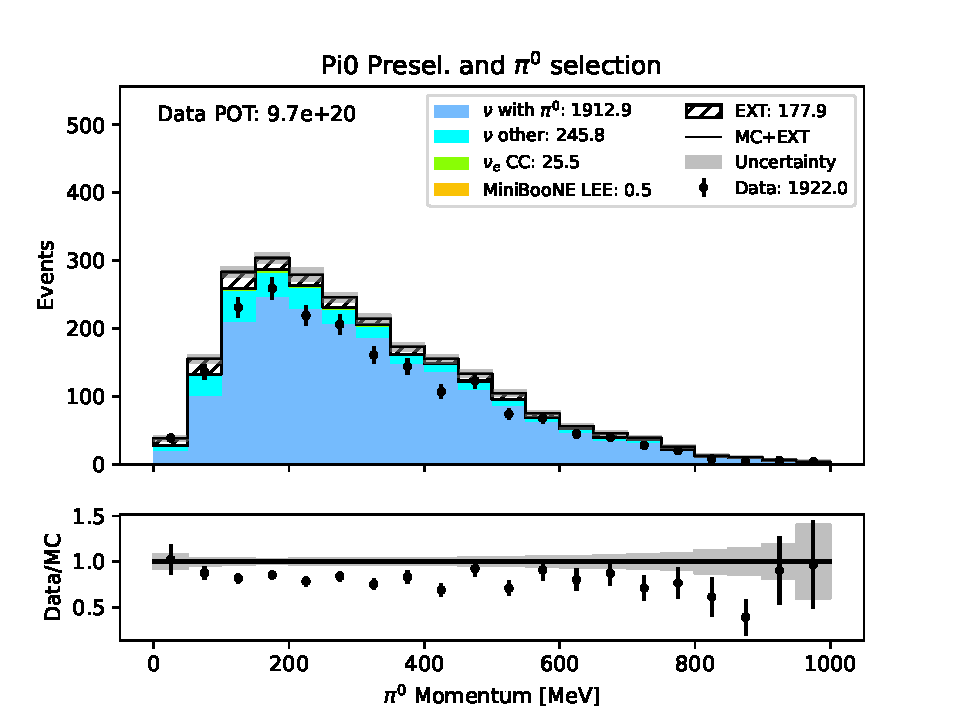
\includegraphics[width=\linewidth]{technote/Sidebands/Figures/TwoShowerSideband/two_shr_sideband_pi0momentum_run1234b4c4d_PI0_PI0.pdf}
        \caption{Reconstructed $\pi^0$ momentum.}
    \end{subfigure}%
    \begin{subfigure}{0.33\linewidth}
        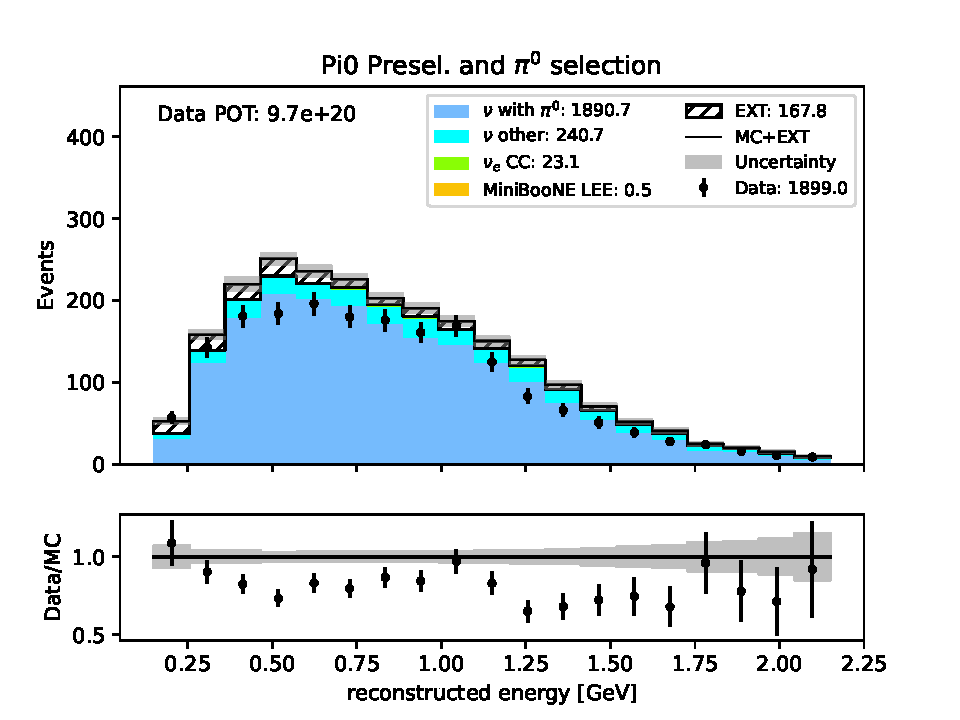
\includegraphics[width=\linewidth]{technote/Sidebands/Figures/TwoShowerSideband/two_shr_sideband_reco_e_run1234b4c4d_PI0_PI0.pdf}
        \caption{Reconstructed neutrino energy.}
    \end{subfigure}
    \caption{Data and MC simulation comparisons after applying the full $\pi^0$ selection from Appendix~\ref{appendix:Pi0Selection} to data from the two shower sideband. Data from runs 1-5 are shown.}
    \label{fig:Pi0SidebandRuns12345}
\end{figure}

\subsection{Near and Far Sidebands}
\label{sec:FarSideband}

The far sidebands are obtained by applying the full event selections for the signal channels, described in Appendix~\ref{appendix:1e0pSelection} and~\ref{appendix:1eNpSelection}, with blindness achieved through inversion of the BDT cuts, or only selecting events with reconstructed energies above the signal region. This approach is illustrated in Figure~\ref{fig:SidebandStructure}, in which the palest green squares represent the far sideband, while the slightly darker green is the near sideband. The definitions are slightly different for the 1e0p and 1eNp event selections.

\begin{figure}[H]
    \centering
    \begin{subfigure}{0.5\linewidth}
        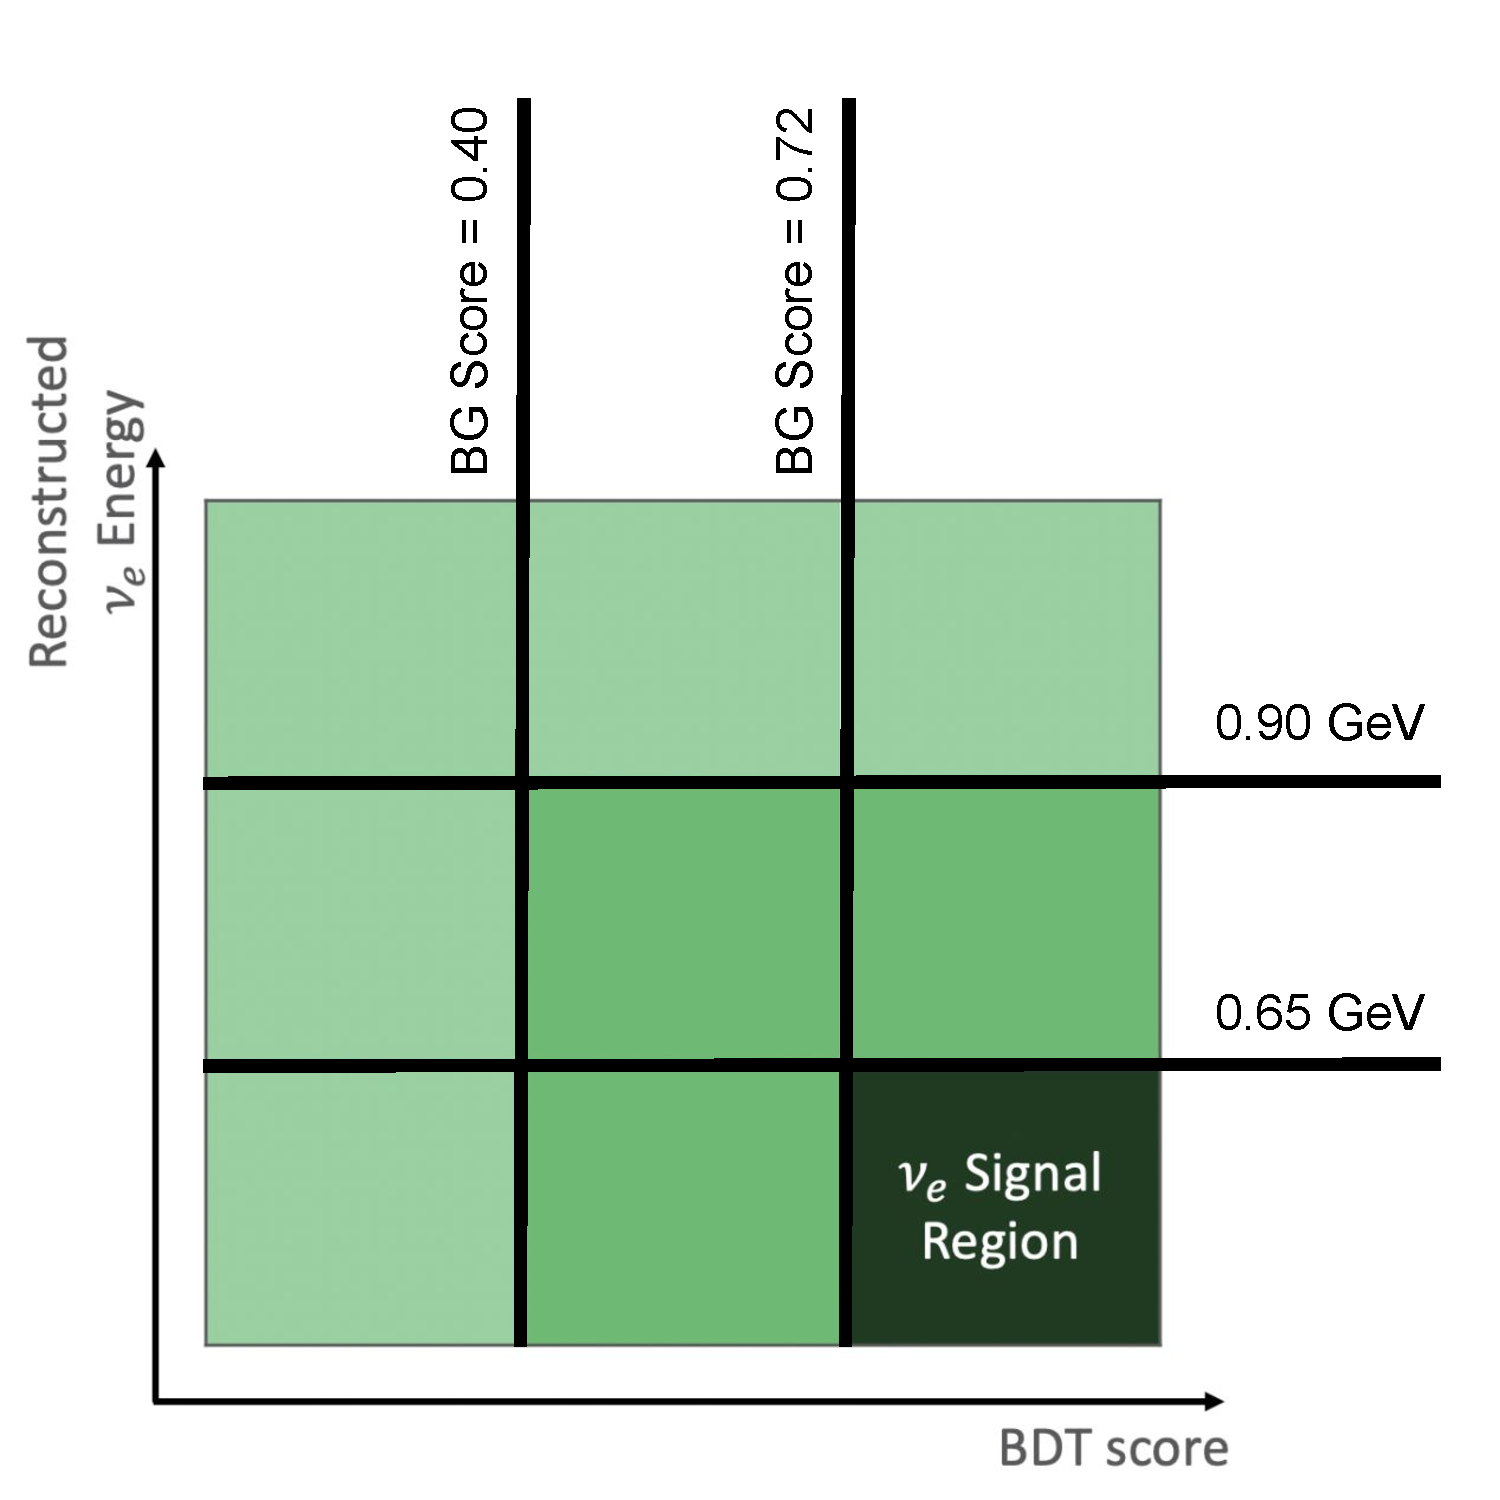
\includegraphics[width=\linewidth]{technote/Sidebands/Figures/ZpNearAndFarSidebands.pdf}
        \caption{For the 1e0p selection.}
    \end{subfigure}%
    \begin{subfigure}{0.5\linewidth}
        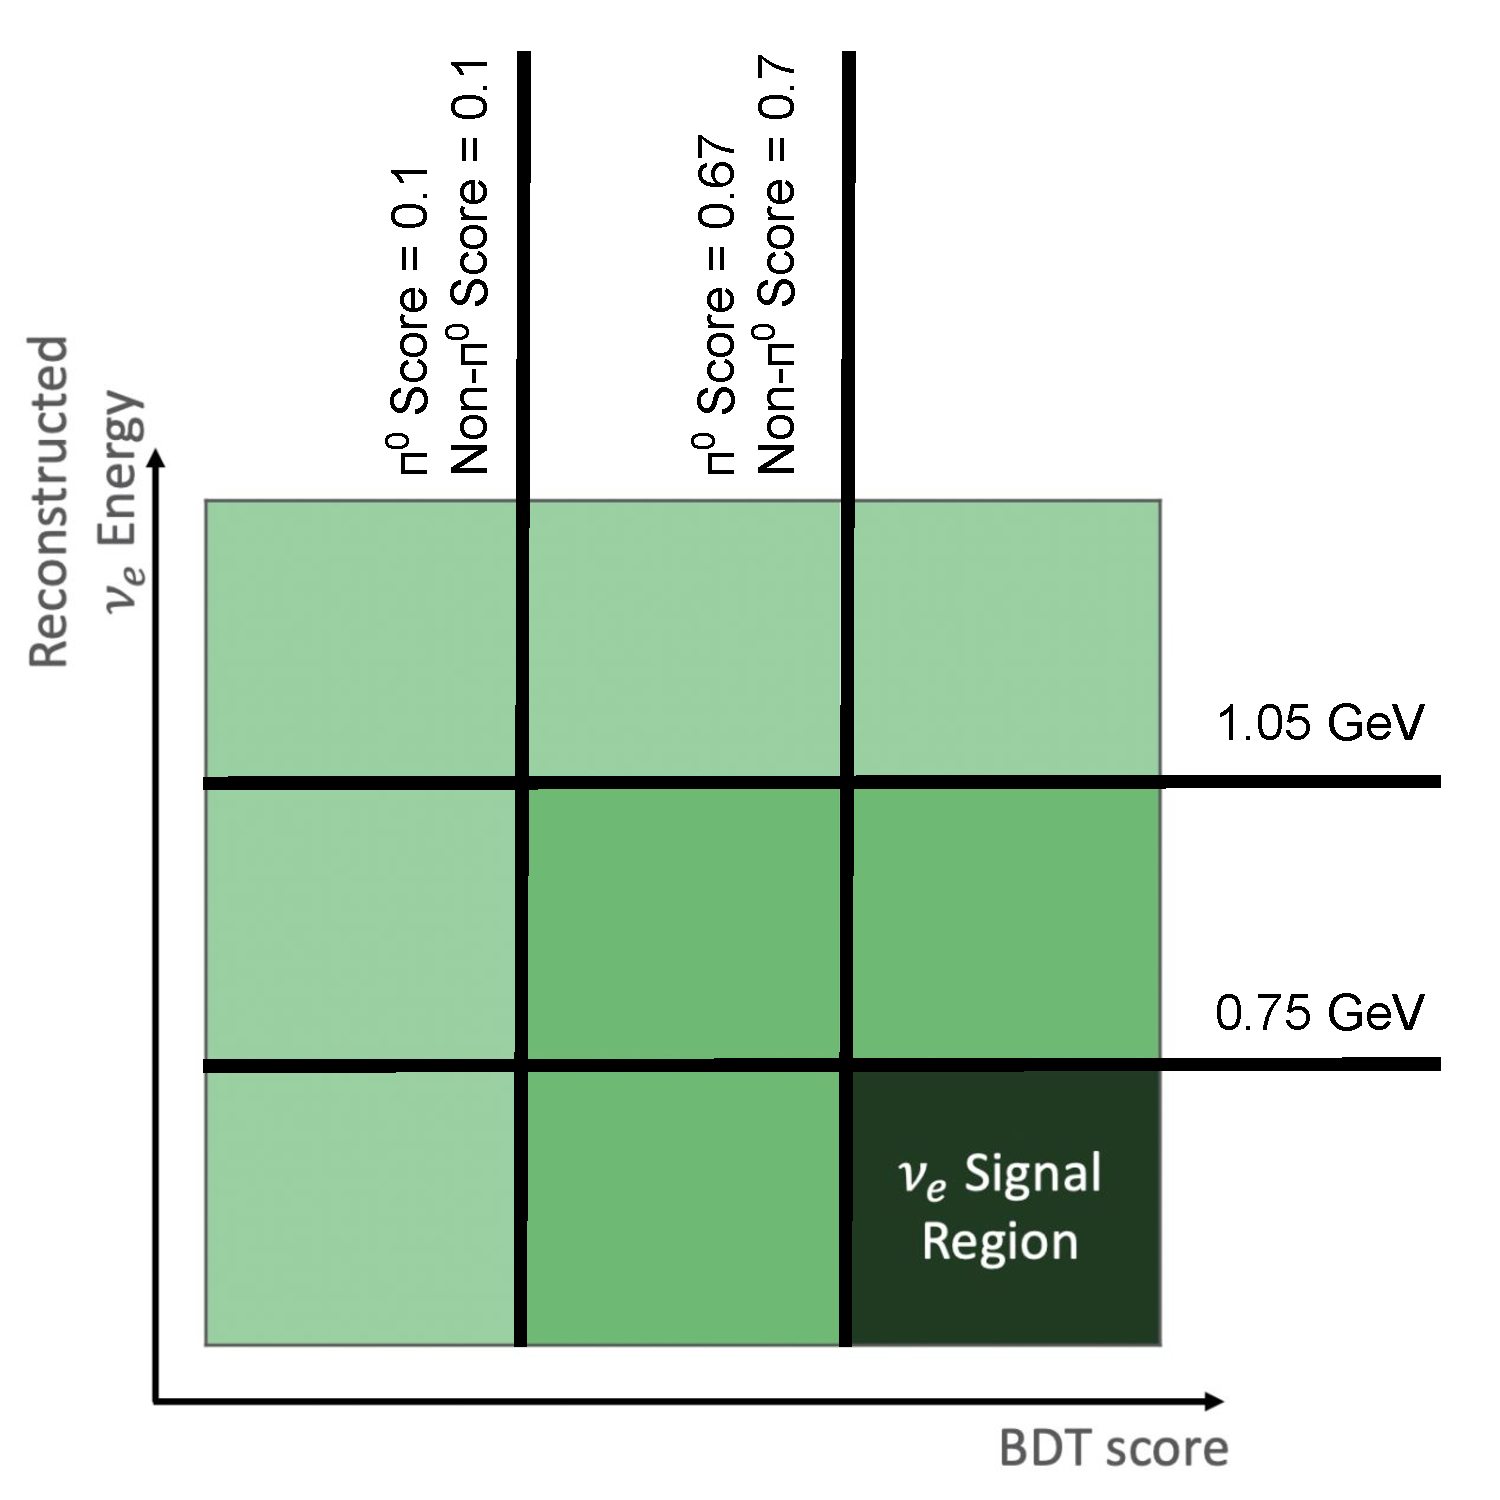
\includegraphics[width=\linewidth]{technote/Sidebands/Figures/NpNearAndFarSidebands.pdf}
        \caption{For the 1eNp selection.}
    \end{subfigure}
    \caption{The structures of the near and far sidebands for the two event selections. The palest green regions represent the far sidebands, while the slightly darker green represents the near sidebands.}
    \label{fig:SidebandStructure}
\end{figure}

\subsection{Shower Energy Sideband}
\label{sec:ShowerEnergySideband}

Two study consistency between the data and MC simulation without applying any selection criteria involving BDTs, we also employ a sideband generated through only selecting events in which the leading shower energy $> 0.75$~GeV. The results of applying the loose event selections to this sideband are shown in Figures~\ref{fig:ShrEnergySideband1eNpRuns123} and~\ref{fig:ShrEnergySideband1e0pRuns123} using data from runs 1-3, and Figures~\ref{fig:ShrEnergySideband1eNpRuns12345} and~\ref{fig:ShrEnergySideband1e0pRuns12345} using data from runs 1-5.

\begin{figure}[H]
    \centering
    \begin{subfigure}{0.5\linewidth}
        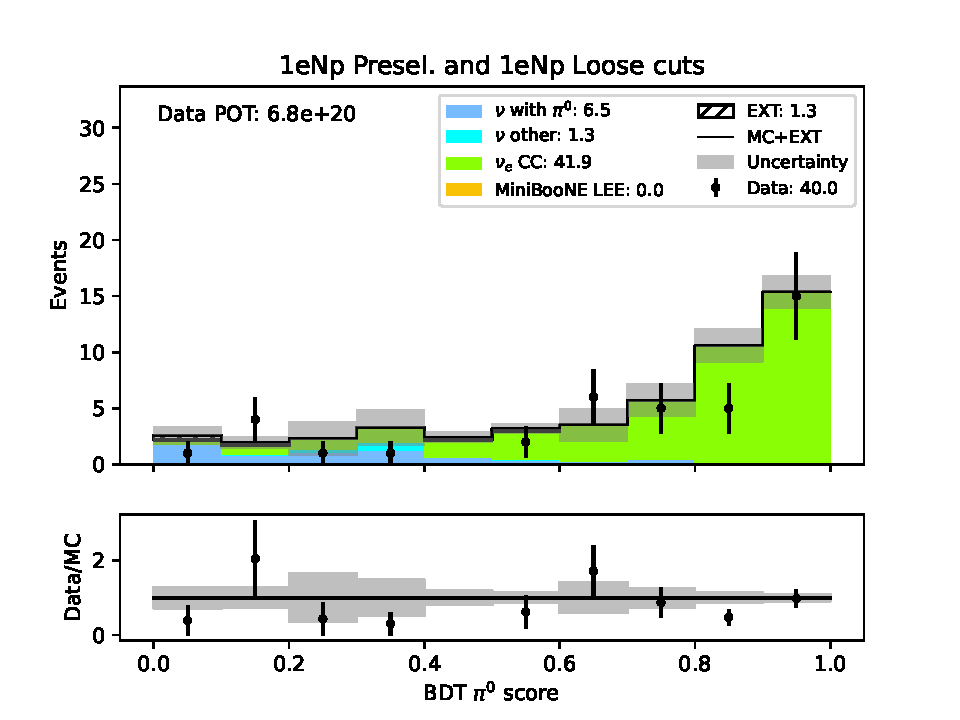
\includegraphics[width=\linewidth]{technote/Sidebands/Figures/ShowerEnergySideband/shr_energy_sideband_pi0_score_run123_NP_NPL.pdf}%
        \caption{$\pi^0$ score.}
    \end{subfigure}%
    \begin{subfigure}{0.5\linewidth}
        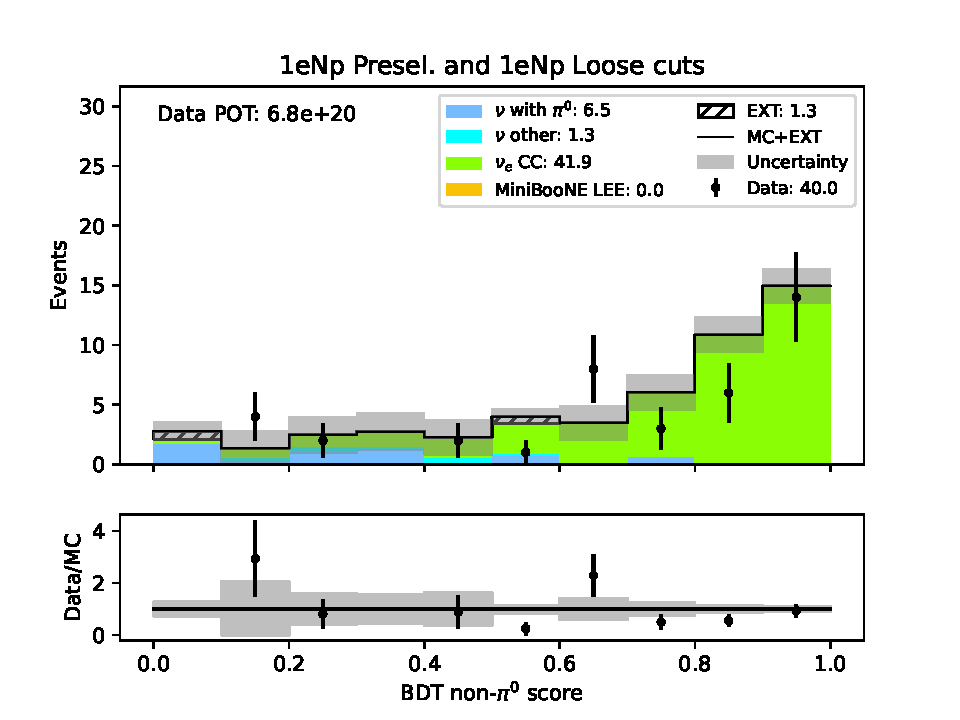
\includegraphics[width=\linewidth]{technote/Sidebands/Figures/ShowerEnergySideband/shr_energy_sideband_nonpi0_score_run123_NP_NPL.pdf}%
        \caption{Non-$\pi^0$ score.}
    \end{subfigure}
    \begin{subfigure}{0.5\linewidth}
        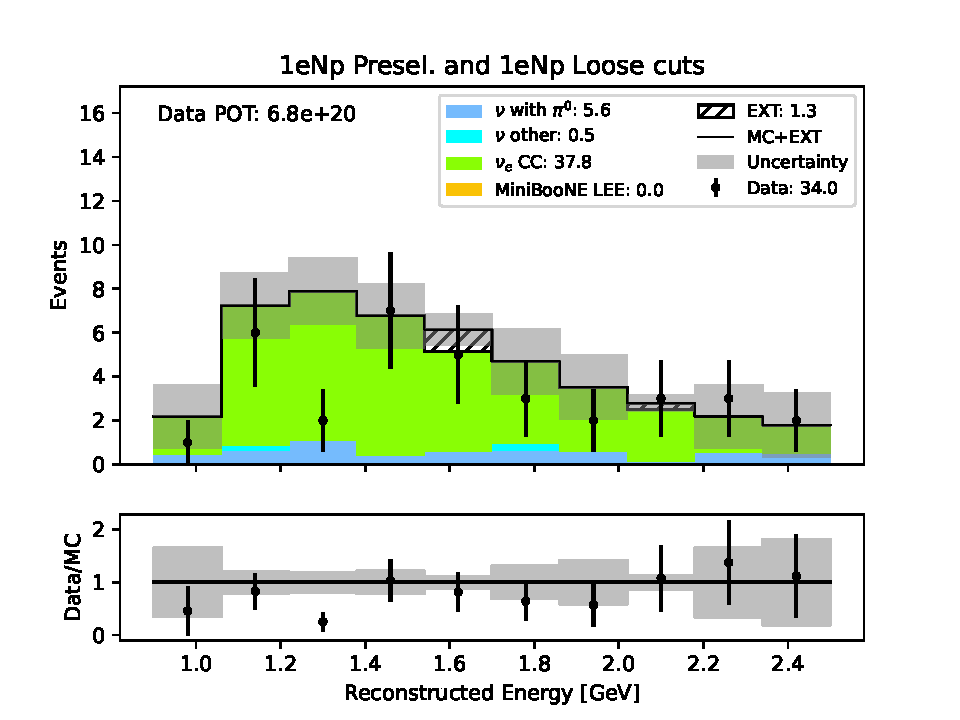
\includegraphics[width=\linewidth]{technote/Sidebands/Figures/ShowerEnergySideband/shr_energy_sideband_reco_e_run123_NP_NPL.pdf}%
        \caption{Reconstructed neutrino energy.}
    \end{subfigure}
    \caption{Results of applying the loose 1eNp event selection to the high shower energy sideband. Data from runs 1, 2, and 3 shown.}
    \label{fig:ShrEnergySideband1eNpRuns123}
\end{figure}

\begin{figure}[H]
    \centering
    \begin{subfigure}{0.5\linewidth}
        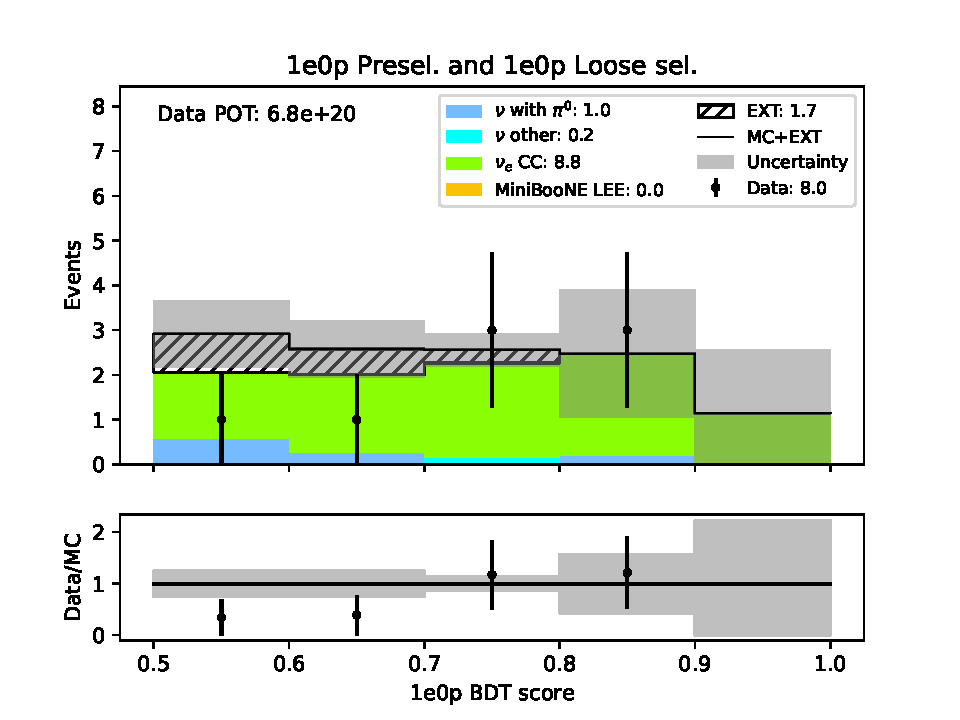
\includegraphics[width=\linewidth]{technote/Sidebands/Figures/ShowerEnergySideband/shr_energy_sideband_bkg_score_run123_ZP_ZPLOOSESEL.pdf}%
        \caption{Background score.}
    \end{subfigure}%
    \begin{subfigure}{0.5\linewidth}
        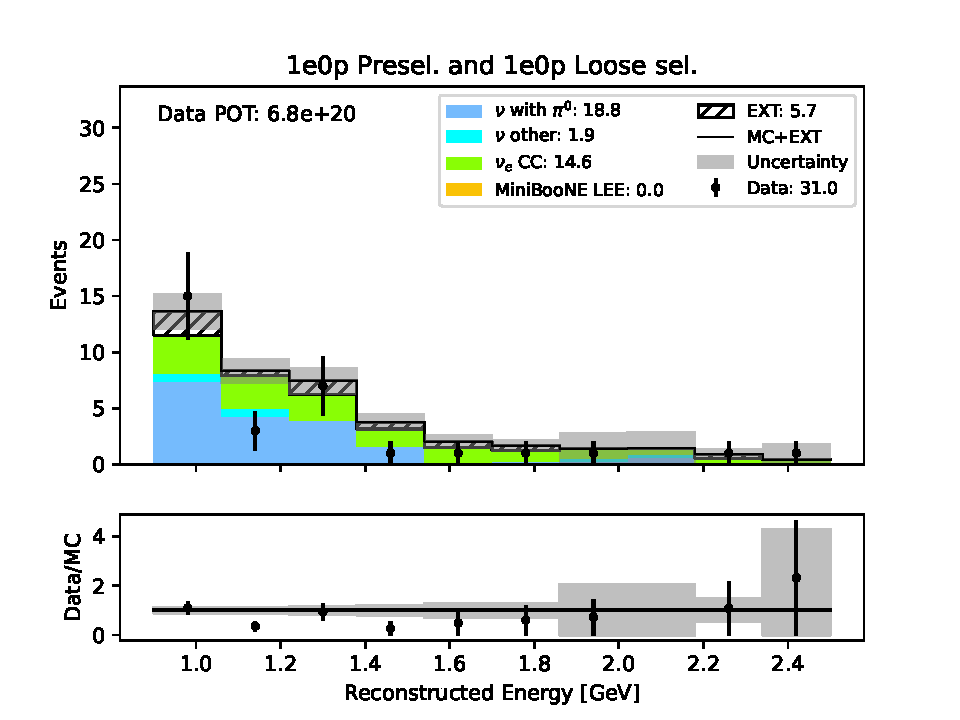
\includegraphics[width=\linewidth]{technote/Sidebands/Figures/ShowerEnergySideband/shr_energy_sideband_reco_e_run123_ZP_ZPLOOSESEL.pdf}%
        \caption{Reconstructed neutrino energy.}
    \end{subfigure}
    \caption{Results of applying the loose 1e0p event selection to the high shower energy sideband. Data from runs 1, 2, and 3 shown.}
    \label{fig:ShrEnergySideband1e0pRuns123}
\end{figure}

\begin{figure}[H]
    \centering
    \begin{subfigure}{0.5\linewidth}
        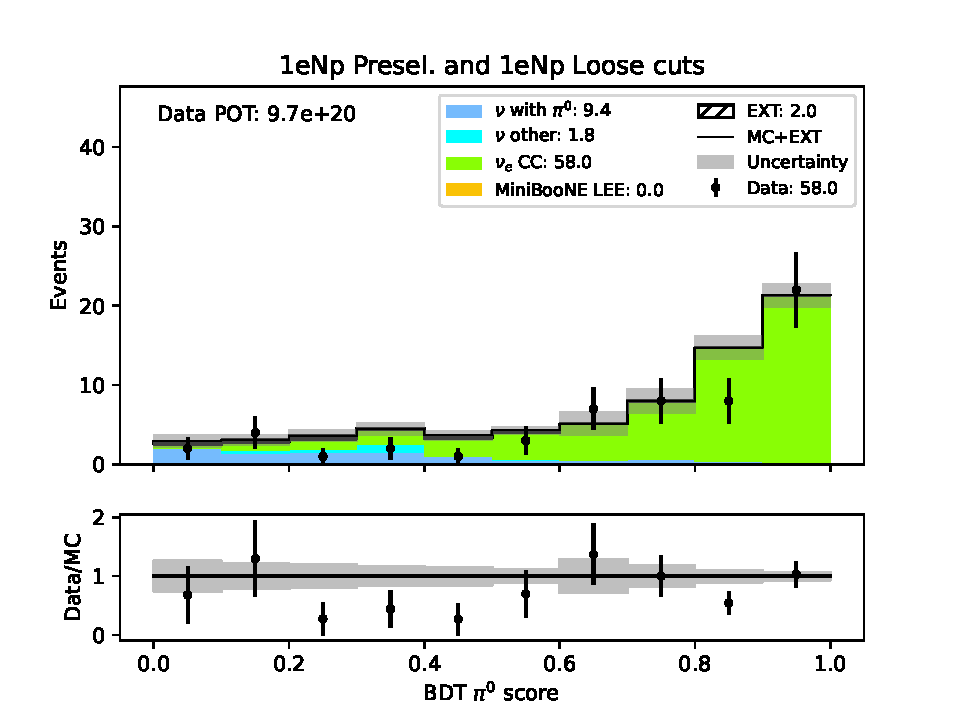
\includegraphics[width=\linewidth]{technote/Sidebands/Figures/ShowerEnergySideband/shr_energy_sideband_pi0_score_run1234b4c4d_NP_NPL.pdf}%
        \caption{$\pi^0$ score.}
    \end{subfigure}%
    \begin{subfigure}{0.5\linewidth}
        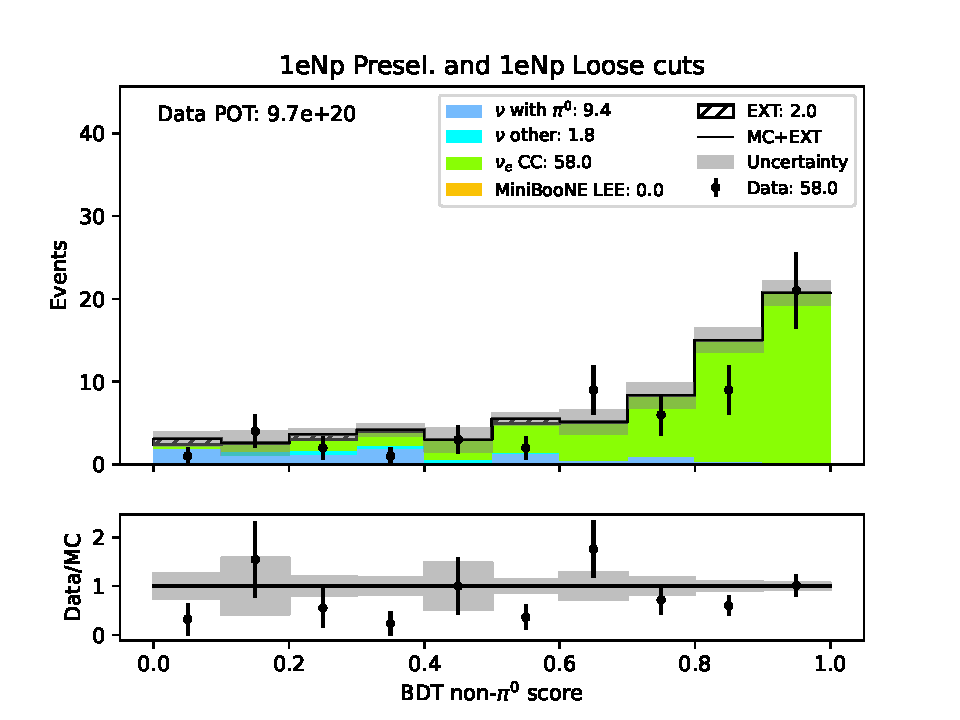
\includegraphics[width=\linewidth]{technote/Sidebands/Figures/ShowerEnergySideband/shr_energy_sideband_nonpi0_score_run1234b4c4d_NP_NPL.pdf}%
        \caption{Non-$\pi^0$ score.}
    \end{subfigure}
    \begin{subfigure}{0.5\linewidth}
        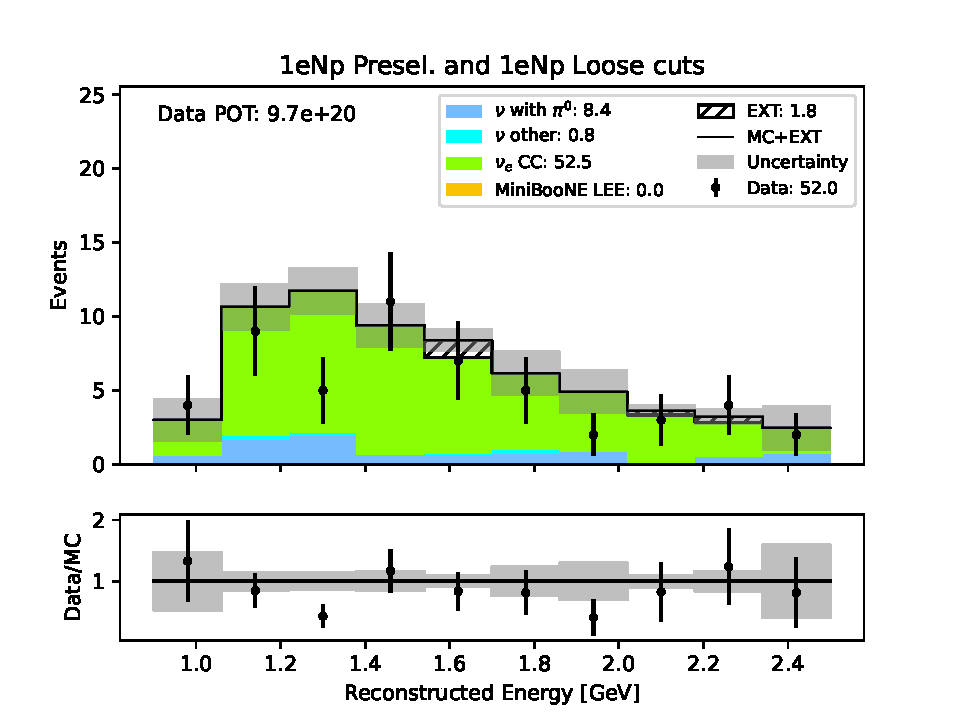
\includegraphics[width=\linewidth]{technote/Sidebands/Figures/ShowerEnergySideband/shr_energy_sideband_reco_e_run1234b4c4d_NP_NPL.pdf}%
        \caption{Reconstructed neutrino energy.}
    \end{subfigure}
    \caption{Results of applying the loose 1eNp event selection to the high shower energy sideband. Data from runs 1-5 shown.}
    \label{fig:ShrEnergySideband1eNpRuns12345}
\end{figure}

\begin{figure}[H]
    \centering
    \begin{subfigure}{0.5\linewidth}
        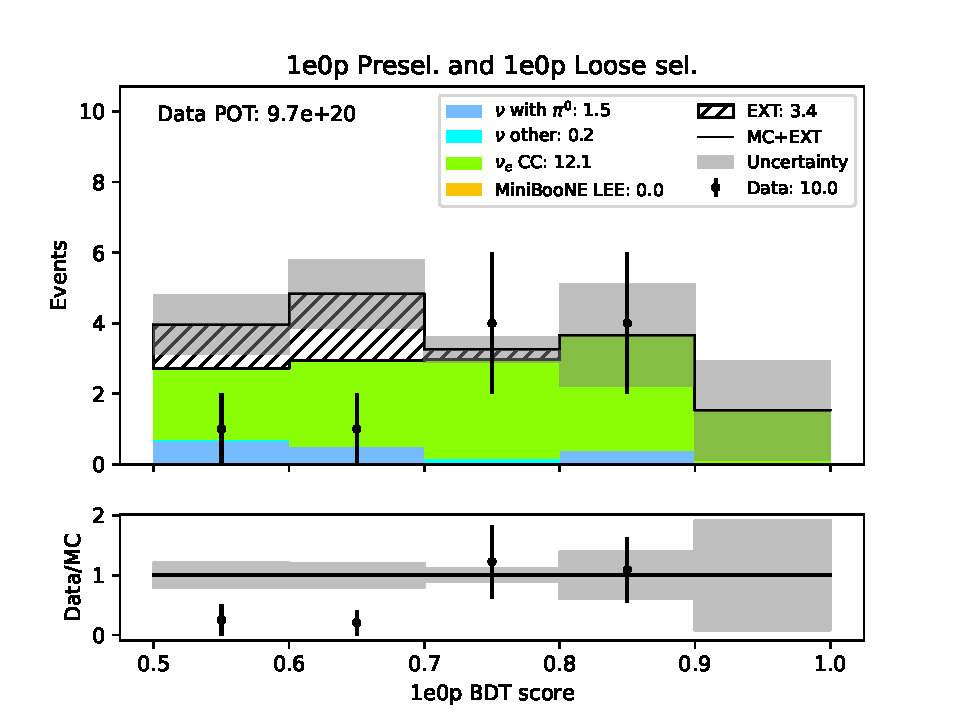
\includegraphics[width=\linewidth]{technote/Sidebands/Figures/ShowerEnergySideband/shr_energy_sideband_bkg_score_run1234b4c4d_ZP_ZPLOOSESEL.pdf}%
        \caption{Background score.}
    \end{subfigure}%
    \begin{subfigure}{0.5\linewidth}
        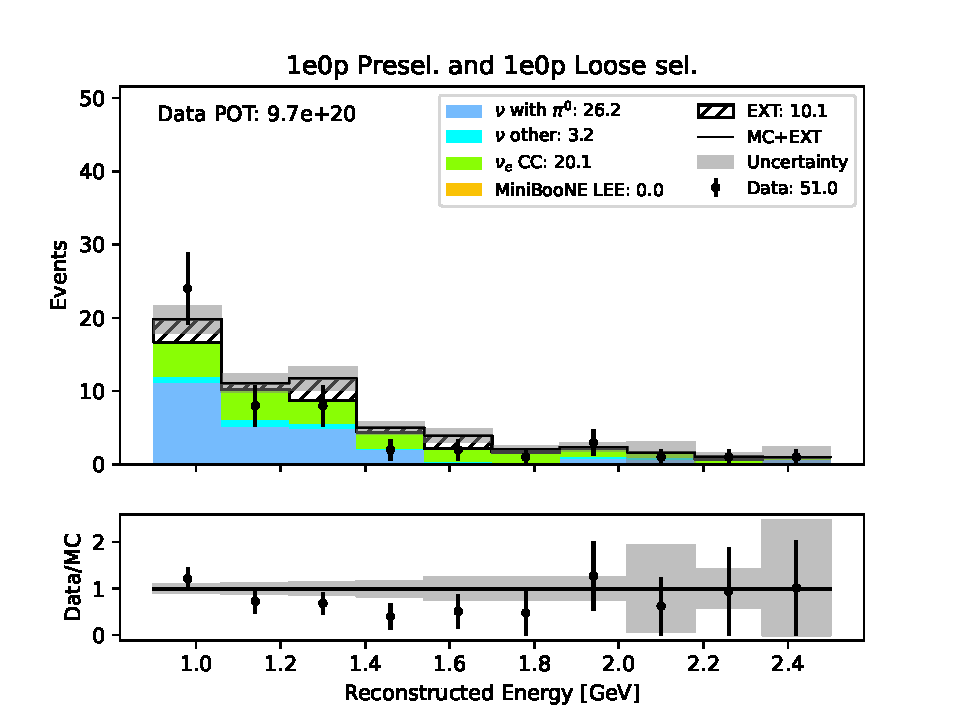
\includegraphics[width=\linewidth]{technote/Sidebands/Figures/ShowerEnergySideband/shr_energy_sideband_reco_e_run1234b4c4d_ZP_ZPLOOSESEL.pdf}%
        \caption{Reconstructed neutrino energy.}
    \end{subfigure}
    \caption{Results of applying the loose 1e0p event selection to the high shower energy sideband. Data from runs 1-5 shown.}
    \label{fig:ShrEnergySideband1e0pRuns12345}
\end{figure}

